\documentclass[20pt]{article}

% set margins and ignore intends
\usepackage[margin=0.9in]{geometry}
\setlength{\parindent}{0pt}

% include graphics
\usepackage{graphicx}

% math stuff
\usepackage{amsmath}
\usepackage{physics}
\usepackage{bbm}

% colors and refs
\usepackage{color}
\usepackage{xcolor}
\usepackage{hyperref}
\usepackage{url}

% definitions and commands
\xdefinecolor{tugreen}{RGB}{132, 184, 24} % define tu green
\def\blue#1{{\color{blue}{#1}}}
\newcommand{\mchapter}[1]{ \begin{center} \color{tugreen!95!black} \LARGE \bf \textbf{#1} \end{center}} % self-made chapters
\newcommand{\msection}[1]{ { \vspace{5mm} \hspace{-6mm} \large \textbf{#1}} \vspace{2mm} } % self-made sections
\newcommand{\mb}{\mathbf} % bold math symbols
\newcommand{\mcaption}[2]{ \\ Figure {#1}: {#2} } % self-made figure captions

% head
% definitions
\font\fb=cmss12   scaled 1200
\font\fc=cmss10   scaled 1000

% head of article
\def\myhead
{

% TU Logo
\vspace*{-1.9cm}
{
    \includegraphics[width=72mm]{tudo_logo.pdf}
}

% CMT 
\vspace*{0.2cm}
{
    \fb
    Condensed Matter Theory\\[1mm]
    Prof.\ Dr.\ G\"otz S. Uhrig\\
}

% address
\vspace*{-3.7cm}
{
    \flushright
    \fc
    \vspace*{7mm}
    TU Dortmund University\\
    \vspace*{-0.6mm}
    Department of Physics / Uhrig Group \\
    \vspace*{-0.6mm}
    44221 Dortmund\\
    \vspace*{-0.6mm}
    Germany\\
    \vspace*{-0.6mm}
    Tel: +49 231 755 3547\\
    \vspace*{-0.6mm}
    Mail: goetz.uhrig@tu-dortmund.de\\
}

}

%%%%%%%%%%%%%%%%%%%%%%%

%%%%%% version 2 (müsste noch umgeschrieben werden) %%%%%%:

%%\vspace*{-0.7cm}
%%\hspace*{-1cm}
%\includegraphics[width=72mm]{tudo_logo.eps}
%%\vspace*{-2.5cm}
%
%
%\fb
%Condensed Matter Theory\\[1mm]
%Prof.\ Dr.\ G\"otz S. Uhrig\\
%\fc \flushright
%Tel/Fax: +49 (0)231 755-3547\,/\,5059\\
%\vspace*{-1mm}
%goetz.uhrig@tu-dortmund.de\\
%}
%
%%\signature{Prof.\ Dr.\ G\"otz S. Uhrig}
%%\place{Dortmund}
%\address{\myhead}
%\date{} % will be ignored
%%\phone{+49 (0)231}{755-3547}
%\backaddress{Condensed Matter Theory, TU Dortmund, D-44221 Dortmund}

%%%%%%%%%%%%%%%%%%%%%%%

\endinput
%%


\begin{document}

% Wer eine Schrift mit Serifen verwendet, kriegt vom Designer
% persönlich auf die Rübe. Darum \sf. 
\sf

% head:
\myhead

% title:
\vspace{2mm}
\mchapter{Collective excitations in correlated quantum materials}
\vspace{-3mm}

% text:
\msection{Scientific context}

Correlated quantum materials have been an everpresent subject of scientific research since the discovery of quantum mechanics.
The BCS-theory of superconductivity from 1957 was the first of its kind to be able to describe the phenomenon, discovered in 1911 by Onnes.
It explains that two electrons form so-called Cooper pairs, which - in contrary to the composing electrons - are bosonic quasiparticles.
If the temperature is below some critical temperature $T_c$ they can condese into a macroscopic occupation of the groundstate.
This mechanism essentially allows for the well-known perfect conductivity.

\msection{Dynamic mean-field theory for spins and applications}


\begin{minipage}{0.44\textwidth}
    The general idea of a mean-field approach is simple. We consider, e.g., a spin lattice consisting of a large number of interacting spins which essentially behave
    the same. Now, we focus on one of these spins and substitute its complex quantum environment by an averaged field which is called \emph{mean-field}. 
    This approximation reduces the intractable lattice problem to a single-site problem. Subsequently, the properties of the mean-field can be linked to those of 
    the remaining spin leading to a so-called \emph{self-consistency problem}. Solving this is the key issue of a mean-field approach.
\end{minipage}
\hspace{0.01\textwidth}
\begin{minipage}{0.54\textwidth}
    \begin{center}
        \includegraphics[width=\textwidth]{images/MFT_sketch.pdf}
        \mcaption{1}{Example for a mean-field approach on a spin lattice.}
    \end{center}
\end{minipage}

\begin{minipage}{0.44\textwidth}
    \begin{center}
        \includegraphics[width=0.8\textwidth]{images/Correlation_sketch.pdf}
        \mcaption{2}{Example for a correlation function of a spin-$1/2$. %At time zero the spin is aligned to its initial position yielding an expectation value of $1/4$. 
        As the time increases, the spin loses the memory of its initial orientation.}
    \end{center}
\end{minipage}
\hspace{0.01\textwidth}
\begin{minipage}{0.54\textwidth}
    In case of our dynamic mean-field theory for spins (spinDMFT), the mean-fields are time-dependent \cite{graes21}. It is developed to compute spin correlation functions such as 
    \begin{align*}
        g^{zz}(t,0) &:= \langle \mb{S}^{z}(t) \mb{S}^{z}(0) \rangle
    \end{align*}
    in the limit of large temperatures. These functions tell us, how much the spin at time $t$ is still correlated to its initial alignment. Correspondingly, they capture the 
    decoherence induced by the spins environment.     
\end{minipage}
\vspace{2mm}

\begin{minipage}{0.65\textwidth}
    A promising application of spinDMFT can be found in the context of nitrogen-vacancy (NV) centers in diamond \cite{jelez06}. They are subject of current research due 
    to their stable spin states up to room temperature which is ideal for many applications such as magnetic sensing \cite{sushk14}. Close to the diamond surface, however, 
    the NV-center coherence is strongly weakened because they are disturbed by other spins stemming from surface defects or adatoms. Understanding 
    the dynamics of these other spins requires considering a large spin ensemble which is where spinDMFT can strike. We are currently collaborating with an experimental 
    group from Boston who measures the correlation functions of the surface defect spins. While spinDMFT itself failed 
    to capture their measurements, we recently obtained good agreement with an extended approach called \emph{Cluster-spinDMFT}.
\end{minipage}
\hspace{0.01\textwidth}
\begin{minipage}{0.35\textwidth}
    \begin{center}
        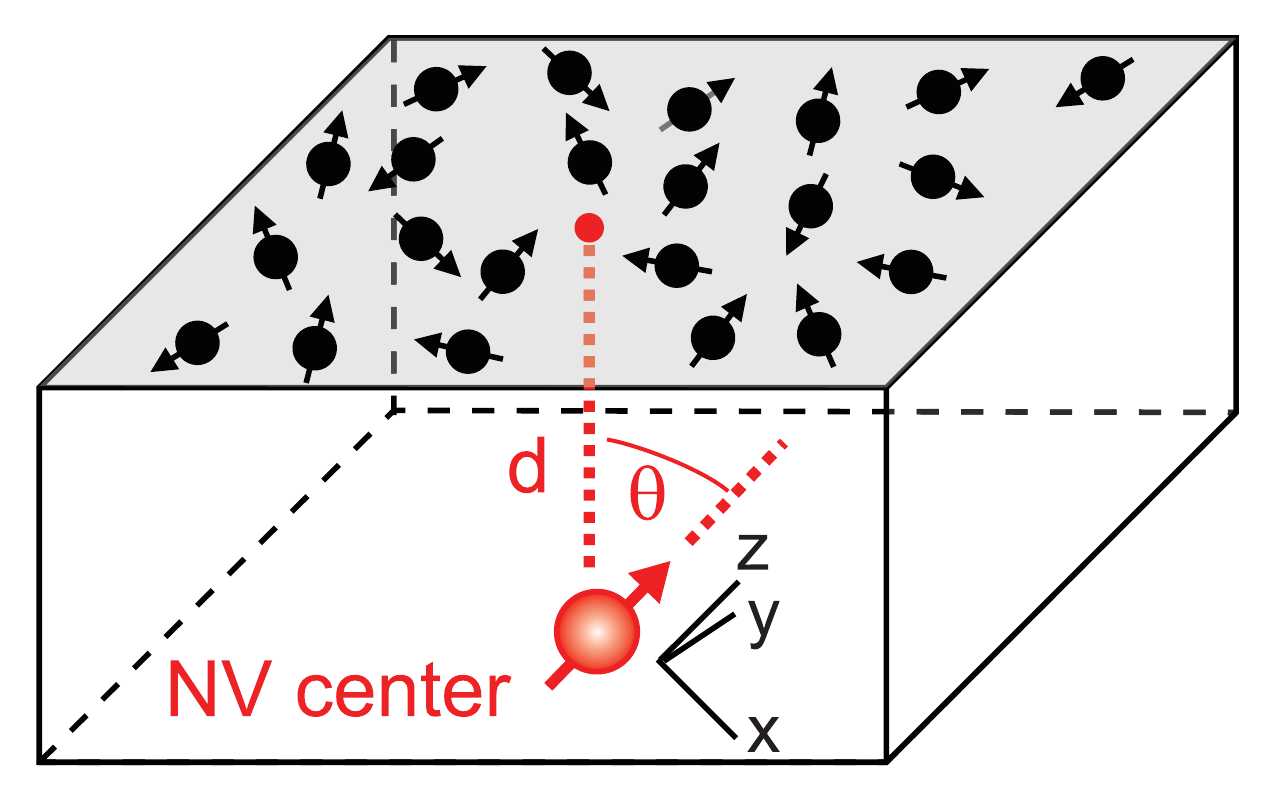
\includegraphics[width=0.8\textwidth]{images/NV_ensemble.png}
        \mcaption{3}{NV-center at a diamond surface with perturbing spins on the surface (black) \cite{rossk14}.}
    \end{center}     
\end{minipage}
\vspace{1.3mm}

It is also possible to extend spinDMFT to external time dependencies. This enables us to introduce pulses to the mean-field simulation and to investigate phenomena such as 
\emph{dynamic decoupling} \cite{uhrig07}. The idea of this is to periodically rotate a considered spin in order to weaken the effects of its environment and, 
hence, to extend its coherence time.

Another potential project is the extension to spatial dependencies. Here, we plan to study how the effects of a pulse propagate through the sample. 
The underlying phenomenon is called spin diffusion \cite{zu21}.

As indicated above, a strong advantage of spinDMFT is its versatility. It can be easily extended to consider complex spin 
configurations, anisotropies, time dependencies and more. Since the theoretical and numerical background has already been established, applying spinDMFT to new 
scenarios becomes more and more important. Here, an internship is a great opportunity.


\msection{Possible tasks during an internship}

Generally, the internship involves mainly \emph{numerical} tasks and \emph{coding}. 
%The work flow for applying the mean-field-approach looks as 
%follows. First, a considered spin model has to be transformed to a mean-field model. Subsequently, the self-consistency conditions derived in the process can be solved with 
%existing code in \textbf{C++}. Sometimes, numerical difficulties arise that demand to change details of the method. In the end, the results can be evaluated to 
%observe exciting new phenomena. 
A specific project could be the investigation of dynamic decoupling in a system comprising a single \emph{spin subject to a Gaussian noise}. Such a project would start
with yourself reading through some literature provided by us so that you understand the fundamental ideas. Subsequently, you would start writing a first simple program in \textbf{C++}, 
that introduces noise, artificial or from a mean-field approach, to a spin. In doing so, you can use existing code fragments from us on some of the required numerical methods. Subsequently, 
you would introduce a pulse sequence such as \emph{UDD} \cite{uhrig07} to the spin in order to enhance its coherence.
One goal of the project could be to find an optimal pulse sequence in dependence of the underlying noise. We emphasize, that this is only \textbf{one} potential project 
and there are many other possibilities. Generally, a little experience 
in \textbf{C++}, \emph{Python} or coding is advantageous. Moreover, knowledge of quantum mechanics is desirable.


\msection{General information}

The chair currently consists of 9 people, that is, 6 PhD students, 1 postdoc as well as Prof. G\"otz S. Uhrig and Prof. Joachim Stolze. The group 
works on a broad range of physical topics such as topological magnonics, non-equilibrium physics, coherence control and more. We have a weekly seminar in which
progress is reported and articles are discussed (Journal Club). Feel free to visit our homepage 
at \url{https://cmt.physik.tu-dortmund.de/uhrig-group/}. 
The methodology and the investigation of collective excitations is the research area of the PhD student Joshua Alth\"user who will also be your supervisor.
You will get your own office space and access to our compute clusters. We do not offer a virtual internship.

% bibliography
\bibliography{lit} 
\bibliographystyle{ieeetr}


\end{document}

